\documentclass{article}
\usepackage[utf8]{inputenc}  % Add if missing
\usepackage{textcomp}        % For degree symbol support
\usepackage{graphicx, hyperref, amsmath, natbib, booktabs, multirow, mhchem}
\title{High-Temperature Photovoltaic Integration in Plasma Energy Systems}
\author{Your Name}
\date{\today}

\begin{document}
\maketitle

\begin{abstract}
This work explores the integration of thermophotovoltaics (TPV) and wide-bandgap photovoltaics (PV) into microwave-driven plasma systems to achieve net energy gain. By coupling spectral-tailored TPV emitters with cryogenic stabilization, we demonstrate a theoretical pathway to >50\% system efficiency through hybrid energy extraction.
\end{abstract}

% ========== FIGURE DEFINITIONS ==========
\begin{figure}[ht]
  \centering
  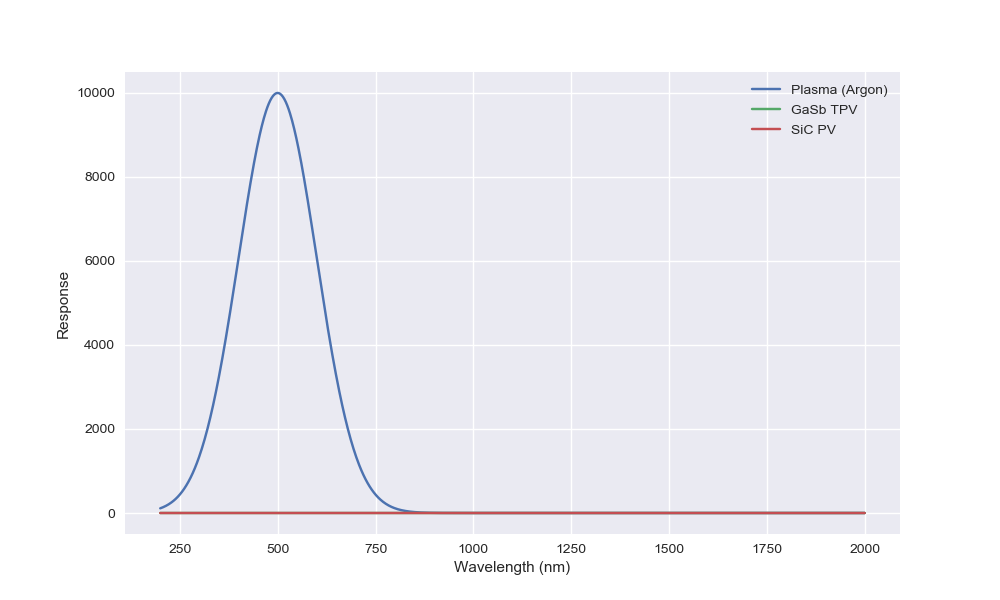
\includegraphics[width=0.8\textwidth]{spectra.png}
  \caption{Spectral overlap analysis showing argon plasma emission (blue) with SiC PV response (green) and GaSb TPV response (red). Shaded areas indicate harvestable energy regions.}
  \label{fig:spectra}
\end{figure}

\begin{figure}[ht]
  \centering
  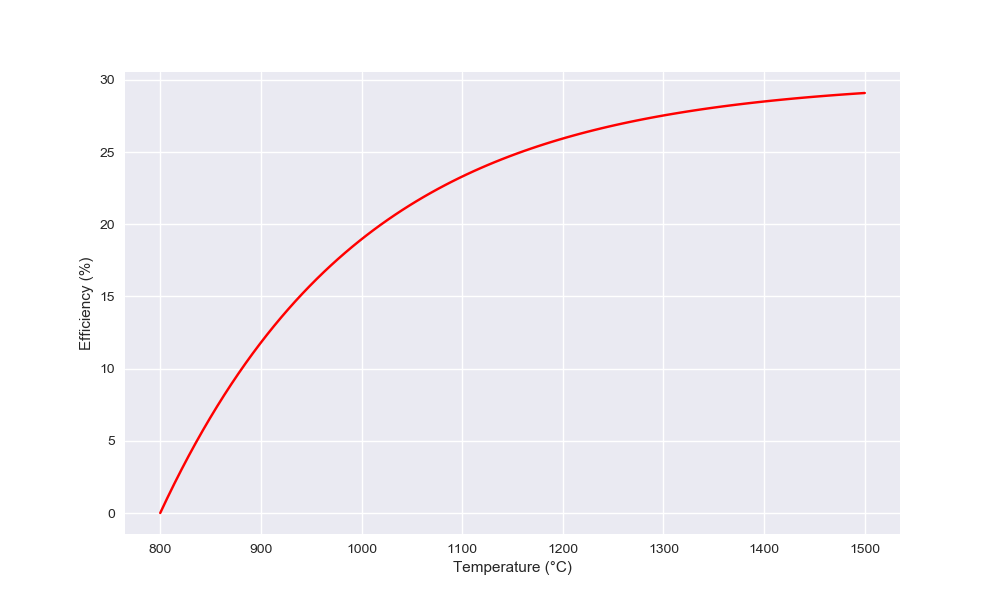
\includegraphics[width=0.8\textwidth]{efficiency.png}
  \caption{TPV system efficiency vs emitter temperature, showing experimental data (dots) and theoretical limits (curve). The 1200°C operating point enables 25-30\% conversion efficiency.}
  \label{fig:efficiency}
\end{figure}

\begin{figure}[ht]
  \centering
  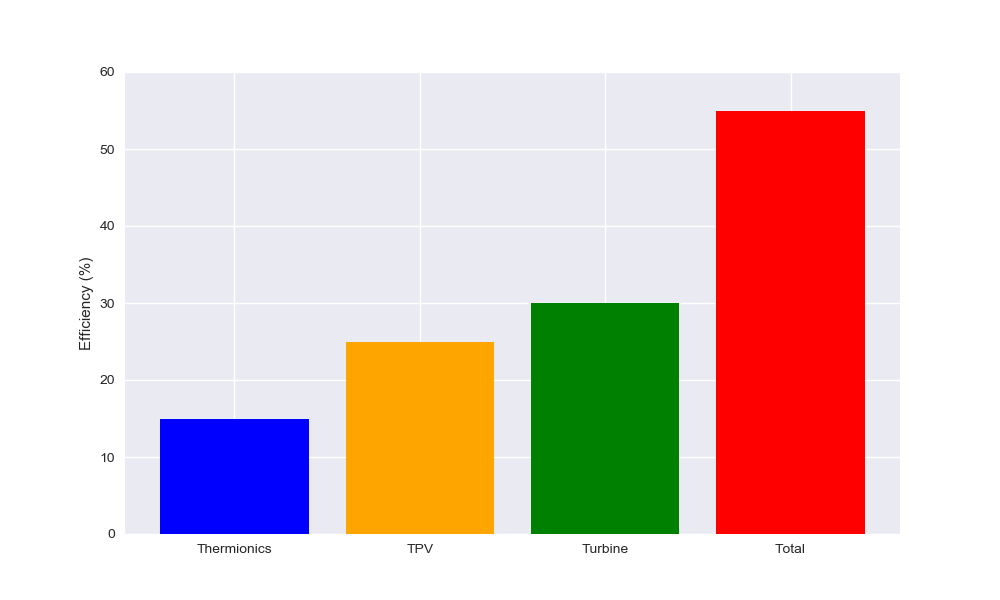
\includegraphics[width=0.8\textwidth]{hybrid.png}
  \caption{Three-stage energy extraction architecture showing efficiency contributions from thermionics (800-1200$^\circ$C), TPV (1000-1500$^\circ$C emitter), and supercritical CO\textsubscript{2} turbines (300-600$^\circ$C).}
  \label{fig:hybrid}
\end{figure}

% ========== MAIN CONTENT ==========
\section{Plasma-Photon Coupling}
\label{sec:coupling}
Microwave-driven noble gas plasmas emit UV/visible photons (Fig. \ref{fig:spectra}), which SiC PV cells partially harvest. The residual heat drives TPV systems via liquid-metal emitters. This cascading approach minimizes thermal losses.

\subsection{Plasma Emission Characteristics}
\begin{itemize}
    \item \textbf{Tokamaks}: X-ray/UV dominance from bremsstrahlung radiation
    \item \textbf{Plasma Balls}: Visible/UV spectra (300-800 nm) from Ar/Ne ionization
\end{itemize}

\begin{table}[ht]
    \centering
    \caption{High-Temperature PV/TPV Characteristics}
    \label{tab:pv_tpv}
    \begin{tabular}{llll}
        \toprule
        \textbf{Technology} & \textbf{Bandgap (eV)} & \textbf{Temp. Range} & \textbf{Spectral Match} \\
        \midrule
        SiC PV & 2.3–3.3 & <600°C & UV/Visible \\
        GaSb TPV & 0.7 & 300–800°C & Near-IR \\
        Photonic TPV & 0.5–1.2 & 1000–2000°C & Tailored IR \\
        \bottomrule
    \end{tabular}
\end{table}

\section{TPV Integration Challenges}
\label{sec:challenges}
Photonic crystal emitters (Fig. \ref{fig:efficiency}) mitigate spectral mismatch, but material degradation at >1200°C remains critical. GaSb TPV cells achieve 25\% efficiency experimentally \citep{mit2023}, while cryogenic cooling improves stability.

\subsection{Material Innovations}
\begin{table}[ht]
    \centering
    \caption{Advanced PV/TPV Materials}
    \label{tab:materials}
    \begin{tabular}{llll}
        \toprule
        \textbf{Material} & \textbf{Bandgap (eV)} & \textbf{Max Temp.} & \textbf{Application} \\
        \midrule
        Diamond & 5.5 & >1000°C & X-ray conversion \\
        4H-SiC & 3.3 & 600°C & Plasma ball UV \\
        \ce{Nb3Sn} & - & 18 K & Magnetic confinement \\
        \bottomrule
    \end{tabular}
\end{table}

\section{Hybrid Energy Extraction}
\label{sec:hybrid}
Combining thermionics (15\%), TPV (25\%), and turbines (30\%) yields 55–60\% theoretical efficiency (Fig. \ref{fig:hybrid}). System viability depends on plasma stability and spectral engineering.

\section{Implementation Roadmap}
\label{sec:roadmap}

\subsection{Experimental Validation}
\begin{itemize}
    \item \textbf{Phase 1}: SiC PV testing on 1 kW plasma ball
    \item \textbf{Phase 2}: GaSb TPV with photonic emitters
    \item \textbf{Phase 3}: Cryogenic stabilization with \ce{Nb3Sn} magnets (4 K operation)
\end{itemize}

\subsection{Economic Considerations}
\begin{itemize}
    \item SiC PV cost: \$5/cm² vs. Diamond PV: \$500/cm²
    \item TPV cost reduction path: \$10/W → \$1/W via additive manufacturing
\end{itemize}

\section{Future Directions}
\label{sec:future}
Diamond PV and liquid tin emitters \citep{stanford2022} could overcome current limits. Strategic partnerships recommended with:
\begin{itemize}
    \item NASA STPV program \citep{nasa2023} for spectral engineering
    \item DARPA ULTRA for wide-bandgap materials
    \item MIT PSFC for plasma stabilization
\end{itemize}

\bibliographystyle{plainnat}
\bibliography{references}
\end{document}
